
%% bare_jrnl.tex
%% V1.3
%% 2007/01/11
%% by Michael Shell
%% see http://www.michaelshell.org/
%% for current contact information.
%%
%% This is a skeleton file demonstrating the use of IEEEtran.cls
%% (requires IEEEtran.cls version 1.7 or later) with an IEEE journal paper.
%%
%% Support sites:
%% http://www.michaelshell.org/tex/ieeetran/
%% http://www.ctan.org/tex-archive/macros/latex/contrib/IEEEtran/
%% and
%% http://www.ieee.org/



% *** Authors should verify (and, if needed, correct) their LaTeX system  ***
% *** with the testflow diagnostic prior to trusting their LaTeX platform ***
% *** with production work. IEEE's font choices can trigger bugs that do  ***
% *** not appear when using other class files.                            ***
% The testflow support page is at:
% http://www.michaelshell.org/tex/testflow/


%%*************************************************************************
%% Legal Notice:
%% This code is offered as-is without any warranty either expressed or
%% implied; without even the implied warranty of MERCHANTABILITY or
%% FITNESS FOR A PARTICULAR PURPOSE!
%% User assumes all risk.
%% In no event shall IEEE or any contributor to this code be liable for
%% any damages or losses, including, but not limited to, incidental,
%% consequential, or any other damages, resulting from the use or misuse
%% of any information contained here.
%%
%% All comments are the opinions of their respective authors and are not
%% necessarily endorsed by the IEEE.
%%
%% This work is distributed under the LaTeX Project Public License (LPPL)
%% ( http://www.latex-project.org/ ) version 1.3, and may be freely used,
%% distributed and modified. A copy of the LPPL, version 1.3, is included
%% in the base LaTeX documentation of all distributions of LaTeX released
%% 2003/12/01 or later.
%% Retain all contribution notices and credits.
%% ** Modified files should be clearly indicated as such, including  **
%% ** renaming them and changing author support contact information. **
%%
%% File list of work: IEEEtran.cls, IEEEtran_HOWTO.pdf, bare_adv.tex,
%%                    bare_conf.tex, bare_jrnl.tex, bare_jrnl_compsoc.tex
%%*************************************************************************

% Note that the a4paper option is mainly intended so that authors in
% countries using A4 can easily print to A4 and see how their papers will
% look in print - the typesetting of the document will not typically be
% affected with changes in paper size (but the bottom and side margins will).
% Use the testflow package mentioned above to verify correct handling of
% both paper sizes by the user's LaTeX system.
%
% Also note that the "draftcls" or "draftclsnofoot", not "draft", option
% should be used if it is desired that the figures are to be displayed in
% draft mode.
%

\documentclass[11pt,draftclsnofoot,onecolumn]{IEEEtran}
%\documentclass[11pt,final,onecolumn]{IEEEtran}
%\documentclass[journal,twosides]{IEEEtran}
 \pagestyle{plain}
%
% If IEEEtran.cls has not been installed into the LaTeX system files,
% manually specify the path to it like:
% \documentclass[journal]{../sty/IEEEtran}





% Some very useful LaTeX packages include:
% (uncomment the ones you want to load)


% *** MISC UTILITY PACKAGES ***
%
%\usepackage{ifpdf}
% Heiko Oberdiek's ifpdf.sty is very useful if you need conditional
% compilation based on whether the output is pdf or dvi.
% usage:
% \ifpdf
%   % pdf code
% \else
%   % dvi code
% \fi
% The latest version of ifpdf.sty can be obtained from:
% http://www.ctan.org/tex-archive/macros/latex/contrib/oberdiek/
% Also, note that IEEEtran.cls V1.7 and later provides a builtin
% \ifCLASSINFOpdf conditional that works the same way.
% When switching from latex to pdflatex and vice-versa, the compiler may
% have to be run twice to clear warning/error messages.






% *** CITATION PACKAGES ***
%
\usepackage{cite}
% cite.sty was written by Donald Arseneau
% V1.6 and later of IEEEtran pre-defines the format of the cite.sty package
% \cite{} output to follow that of IEEE. Loading the cite package will
% result in citation numbers being automatically sorted and properly
% "compressed/ranged". e.g., [1], [9], [2], [7], [5], [6] without using
% cite.sty will become [1], [2], [5]--[7], [9] using cite.sty. cite.sty's
% \cite will automatically add leading space, if needed. Use cite.sty's
% noadjust option (cite.sty V3.8 and later) if you want to turn this off.
% cite.sty is already installed on most LaTeX systems. Be sure and use
% version 4.0 (2003-05-27) and later if using hyperref.sty. cite.sty does
% not currently provide for hyperlinked citations.
% The latest version can be obtained at:
% http://www.ctan.org/tex-archive/macros/latex/contrib/cite/
% The documentation is contained in the cite.sty file itself.






% *** GRAPHICS RELATED PACKAGES ***
%
\ifCLASSINFOpdf
  % \usepackage[pdftex]{graphicx}
  % declare the path(s) where your graphic files are
  % \graphicspath{{../pdf/}{../jpeg/}}
  % and their extensions so you won't have to specify these with
  % every instance of \includegraphics
  % \DeclareGraphicsExtensions{.pdf,.jpeg,.png}
\else
  % or other class option (dvipsone, dvipdf, if not using dvips). graphicx
  % will default to the driver specified in the system graphics.cfg if no
  % driver is specified.
  % \usepackage[dvips]{graphicx}
  % declare the path(s) where your graphic files are
  % \graphicspath{{../eps/}}
  % and their extensions so you won't have to specify these with
  % every instance of \includegraphics
  % \DeclareGraphicsExtensions{.eps}
\fi
% graphicx was written by David Carlisle and Sebastian Rahtz. It is
% required if you want graphics, photos, etc. graphicx.sty is already
% installed on most LaTeX systems. The latest version and documentation can
% be obtained at:
% http://www.ctan.org/tex-archive/macros/latex/required/graphics/
% Another good source of documentation is "Using Imported Graphics in
% LaTeX2e" by Keith Reckdahl which can be found as epslatex.ps or
% epslatex.pdf at: http://www.ctan.org/tex-archive/info/
%
% latex, and pdflatex in dvi mode, support graphics in encapsulated
% postscript (.eps) format. pdflatex in pdf mode supports graphics
% in .pdf, .jpeg, .png and .mps (metapost) formats. Users should ensure
% that all non-photo figures use a vector format (.eps, .pdf, .mps) and
% not a bitmapped formats (.jpeg, .png). IEEE frowns on bitmapped formats
% which can result in "jaggedy"/blurry rendering of lines and letters as
% well as large increases in file sizes.
%
% You can find documentation about the pdfTeX application at:
% http://www.tug.org/applications/pdftex





% *** MATH PACKAGES ***
%
%\usepackage[cmex10]{amsmath}
% A popular package from the American Mathematical Society that provides
% many useful and powerful commands for dealing with mathematics. If using
% it, be sure to load this package with the cmex10 option to ensure that
% only type 1 fonts will utilized at all point sizes. Without this option,
% it is possible that some math symbols, particularly those within
% footnotes, will be rendered in bitmap form which will result in a
% document that can not be IEEE Xplore compliant!
%
% Also, note that the amsmath package sets \interdisplaylinepenalty to 10000
% thus preventing page breaks from occurring within multiline equations. Use:
%\interdisplaylinepenalty=2500
% after loading amsmath to restore such page breaks as IEEEtran.cls normally
% does. amsmath.sty is already installed on most LaTeX systems. The latest
% version and documentation can be obtained at:
% http://www.ctan.org/tex-archive/macros/latex/required/amslatex/math/





% *** SPECIALIZED LIST PACKAGES ***
%
%\usepackage{algorithmic}
% algorithmic.sty was written by Peter Williams and Rogerio Brito.
% This package provides an algorithmic environment fo describing algorithms.
% You can use the algorithmic environment in-text or within a figure
% environment to provide for a floating algorithm. Do NOT use the algorithm
% floating environment provided by algorithm.sty (by the same authors) or
% algorithm2e.sty (by Christophe Fiorio) as IEEE does not use dedicated
% algorithm float types and packages that provide these will not provide
% correct IEEE style captions. The latest version and documentation of
% algorithmic.sty can be obtained at:
% http://www.ctan.org/tex-archive/macros/latex/contrib/algorithms/
% There is also a support site at:
% http://algorithms.berlios.de/index.html
% Also of interest may be the (relatively newer and more customizable)
% algorithmicx.sty package by Szasz Janos:
% http://www.ctan.org/tex-archive/macros/latex/contrib/algorithmicx/




% *** ALIGNMENT PACKAGES ***
%
%\usepackage{array}
% Frank Mittelbach's and David Carlisle's array.sty patches and improves
% the standard LaTeX2e array and tabular environments to provide better
% appearance and additional user controls. As the default LaTeX2e table
% generation code is lacking to the point of almost being broken with
% respect to the quality of the end results, all users are strongly
% advised to use an enhanced (at the very least that provided by array.sty)
% set of table tools. array.sty is already installed on most systems. The
% latest version and documentation can be obtained at:
% http://www.ctan.org/tex-archive/macros/latex/required/tools/


%\usepackage{mdwmath}
%\usepackage{mdwtab}
% Also highly recommended is Mark Wooding's extremely powerful MDW tools,
% especially mdwmath.sty and mdwtab.sty which are used to format equations
% and tables, respectively. The MDWtools set is already installed on most
% LaTeX systems. The lastest version and documentation is available at:
% http://www.ctan.org/tex-archive/macros/latex/contrib/mdwtools/


% IEEEtran contains the IEEEeqnarray family of commands that can be used to
% generate multiline equations as well as matrices, tables, etc., of high
% quality.


%\usepackage{eqparbox}
% Also of notable interest is Scott Pakin's eqparbox package for creating
% (automatically sized) equal width boxes - aka "natural width parboxes".
% Available at:
% http://www.ctan.org/tex-archive/macros/latex/contrib/eqparbox/





% *** SUBFIGURE PACKAGES ***
%\usepackage[tight,footnotesize]{subfigure}
% subfigure.sty was written by Steven Douglas Cochran. This package makes it
% easy to put subfigures in your figures. e.g., "Figure 1a and 1b". For IEEE
% work, it is a good idea to load it with the tight package option to reduce
% the amount of white space around the subfigures. subfigure.sty is already
% installed on most LaTeX systems. The latest version and documentation can
% be obtained at:
% http://www.ctan.org/tex-archive/obsolete/macros/latex/contrib/subfigure/
% subfigure.sty has been superceeded by subfig.sty.



%\usepackage[caption=false]{caption}
%\usepackage[font=footnotesize]{subfig}
% subfig.sty, also written by Steven Douglas Cochran, is the modern
% replacement for subfigure.sty. However, subfig.sty requires and
% automatically loads Axel Sommerfeldt's caption.sty which will override
% IEEEtran.cls handling of captions and this will result in nonIEEE style
% figure/table captions. To prevent this problem, be sure and preload
% caption.sty with its "caption=false" package option. This is will preserve
% IEEEtran.cls handing of captions. Version 1.3 (2005/06/28) and later
% (recommended due to many improvements over 1.2) of subfig.sty supports
% the caption=false option directly:
%\usepackage[caption=false,font=footnotesize]{subfig}
%
% The latest version and documentation can be obtained at:
% http://www.ctan.org/tex-archive/macros/latex/contrib/subfig/
% The latest version and documentation of caption.sty can be obtained at:
% http://www.ctan.org/tex-archive/macros/latex/contrib/caption/




% *** FLOAT PACKAGES ***
%
%\usepackage{fixltx2e}
% fixltx2e, the successor to the earlier fix2col.sty, was written by
% Frank Mittelbach and David Carlisle. This package corrects a few problems
% in the LaTeX2e kernel, the most notable of which is that in current
% LaTeX2e releases, the ordering of single and double column floats is not
% guaranteed to be preserved. Thus, an unpatched LaTeX2e can allow a
% single column figure to be placed prior to an earlier double column
% figure. The latest version and documentation can be found at:
% http://www.ctan.org/tex-archive/macros/latex/base/



%\usepackage{stfloats}
% stfloats.sty was written by Sigitas Tolusis. This package gives LaTeX2e
% the ability to do double column floats at the bottom of the page as well
% as the top. (e.g., "\begin{figure*}[!b]" is not normally possible in
% LaTeX2e). It also provides a command:
%\fnbelowfloat
% to enable the placement of footnotes below bottom floats (the standard
% LaTeX2e kernel puts them above bottom floats). This is an invasive package
% which rewrites many portions of the LaTeX2e float routines. It may not work
% with other packages that modify the LaTeX2e float routines. The latest
% version and documentation can be obtained at:
% http://www.ctan.org/tex-archive/macros/latex/contrib/sttools/
% Documentation is contained in the stfloats.sty comments as well as in the
% presfull.pdf file. Do not use the stfloats baselinefloat ability as IEEE
% does not allow \baselineskip to stretch. Authors submitting work to the
% IEEE should note that IEEE rarely uses double column equations and
% that authors should try to avoid such use. Do not be tempted to use the
% cuted.sty or midfloat.sty packages (also by Sigitas Tolusis) as IEEE does
% not format its papers in such ways.


%\ifCLASSOPTIONcaptionsoff
%  \usepackage[nomarkers]{endfloat}
% \let\MYoriglatexcaption\caption
% \renewcommand{\caption}[2][\relax]{\MYoriglatexcaption[#2]{#2}}
%\fi
% endfloat.sty was written by James Darrell McCauley and Jeff Goldberg.
% This package may be useful when used in conjunction with IEEEtran.cls'
% captionsoff option. Some IEEE journals/societies require that submissions
% have lists of figures/tables at the end of the paper and that
% figures/tables without any captions are placed on a page by themselves at
% the end of the document. If needed, the draftcls IEEEtran class option or
% \CLASSINPUTbaselinestretch interface can be used to increase the line
% spacing as well. Be sure and use the nomarkers option of endfloat to
% prevent endfloat from "marking" where the figures would have been placed
% in the text. The two hack lines of code above are a slight modification of
% that suggested by in the endfloat docs (section 8.3.1) to ensure that
% the full captions always appear in the list of figures/tables - even if
% the user used the short optional argument of \caption[]{}.
% IEEE papers do not typically make use of \caption[]'s optional argument,
% so this should not be an issue. A similar trick can be used to disable
% captions of packages such as subfig.sty that lack options to turn off
% the subcaptions:
% For subfig.sty:
% \let\MYorigsubfloat\subfloat
% \renewcommand{\subfloat}[2][\relax]{\MYorigsubfloat[]{#2}}
% For subfigure.sty:
% \let\MYorigsubfigure\subfigure
% \renewcommand{\subfigure}[2][\relax]{\MYorigsubfigure[]{#2}}
% However, the above trick will not work if both optional arguments of
% the \subfloat/subfig command are used. Furthermore, there needs to be a
% description of each subfigure *somewhere* and endfloat does not add
% subfigure captions to its list of figures. Thus, the best approach is to
% avoid the use of subfigure captions (many IEEE journals avoid them anyway)
% and instead reference/explain all the subfigures within the main caption.
% The latest version of endfloat.sty and its documentation can obtained at:
% http://www.ctan.org/tex-archive/macros/latex/contrib/endfloat/
%
% The IEEEtran \ifCLASSOPTIONcaptionsoff conditional can also be used
% later in the document, say, to conditionally put the References on a
% page by themselves.





% *** PDF, URL AND HYPERLINK PACKAGES ***
%
%\usepackage{url}
% url.sty was written by Donald Arseneau. It provides better support for
% handling and breaking URLs. url.sty is already installed on most LaTeX
% systems. The latest version can be obtained at:
% http://www.ctan.org/tex-archive/macros/latex/contrib/misc/
% Read the url.sty source comments for usage information. Basically,
% \url{my_url_here}.





% *** Do not adjust lengths that control margins, column widths, etc. ***
% *** Do not use packages that alter fonts (such as pslatex).         ***
% There should be no need to do such things with IEEEtran.cls V1.6 and later.
% (Unless specifically asked to do so by the journal or conference you plan
% to submit to, of course. )

\usepackage{graphicx}


\usepackage[caption=false,font=footnotesize]{subfig}
%\captionsetup[subfigure]{margin=0pt, justification=centering, singlelinecheck=false}
\graphicspath{{figures/}}
%\usepackage{subfigure}
%\usepackage{epstopdf}
\DeclareGraphicsExtensions{.pdf,.jpeg,.png}
\usepackage{morefloats}
\usepackage{amsmath}
\newtheorem{defn}{Definition}
%\newtheorem{prop}[defn]{Proposition}
\newtheorem{thm}{Theorem}
%\newtheorem{cor}[defn]{Corollary}
%\usepackage{algorithmic}
\usepackage{array}
%\usepackage{mdwmath}
%\usepackage{mdwtab}
%\usepackage{eqparbox}
\usepackage{url}
% \url{my_url_here}.
\usepackage{parskip}
\setlength{\parskip}{\baselineskip}
\setlength{\parindent}{10pt}

% correct bad hyphenation here
\renewcommand{\baselinestretch}{0.95}
\hyphenation{op-tical net-works semi-conduc-tor pa-ckets}


\begin{document}
%
% paper title
%\title{Secure Network-based IP Mobility Scheme for Vehicular Communications Networks}
%\title{Secure Network-based IP Mobility in Multi-hop VANET}
%\title{A Multi-hop Authenticated Proxy Mobile IP Scheme for Asymmetric I2V Communications}
\title{Communication Technologies and Routing in AMI Networks: a Survey}
%
%
% author names and IEEE memberships
% note positions of commas and nonbreaking spaces ( ~ ) LaTeX will not break
% a structure at a ~ so this keeps an author's name from being broken across
% two lines.
% use \thanks{} to gain access to the first footnote area
% a separate \thanks must be used for each paragraph as LaTeX2e's \thanks
% was not built to handle multiple paragraphs
%

\author{Diego F. Ram\'{i}rez, 
			 Sandra~C\'{e}spedes\\%
			 Department of Information and Communication Technologies\\%
			 Icesi University, Cali, Colombia\\%
			 Email: \{\textit{dframirez,scespedes}\}\textit{@icesi.edu.co}}
% <-this % stops a space
%\thanks{D. Ram\'{i}rez and S. C\'{e}spedes are with the 
%Department of Information and Communication Technologies, Icesi University, Cali, Colombia. Email: \{dframirez,slcesped\}@icesi.edu.co}}%

% note the % following the last \IEEEmembership and also \thanks -
% these prevent an unwanted space from occurring between the last author name
% and the end of the author line. i.e., if you had this:
%
% \author{....lastname \thanks{...} \thanks{...} }
%                     ^------------^------------^----Do not want these spaces!
%
% a space would be appended to the last name and could cause every name on that
% line to be shifted left slightly. This is one of those "LaTeX things". For
% instance, "\textbf{A} \textbf{B}" will typeset as "A B" not "AB". To get
% "AB" then you have to do: "\textbf{A}\textbf{B}"
% \thanks is no different in this regard, so shield the last } of each \thanks
% that ends a line with a % and do not let a space in before the next \thanks.
% Spaces after \IEEEmembership other than the last one are OK (and needed) as
% you are supposed to have spaces between the names. For what it is worth,
% this is a minor point as most people would not even notice if the said evil
% space somehow managed to creep in.



% The paper headers
%\markboth{IEEE Transactions on Vehicular Technology,~Vol.~XX, No.~XX}{C\'{e}spedes \MakeLowercase{\textit{et al.}}: A Multi-hop Authenticated Proxy Mobile IP Scheme for Asymmetric VANET}
% The only time the second header will appear is for the odd numbered pages
% after the title page when using the twoside option.
%
% *** Note that you probably will NOT want to include the author's ***
% *** name in the headers of peer review papers.                   ***
% You can use \ifCLASSOPTIONpeerreview for conditional compilation here if
% you desire.




% If you want to put a publisher's ID mark on the page you can do it like
% this:
%\IEEEpubid{0000--0000/00\$00.00~\copyright~2007 IEEE}
% Remember, if you use this you must call \IEEEpubidadjcol in the second
% column for its text to clear the IEEEpubid mark.



% use for special paper notices
%\IEEEspecialpapernotice{(Invited Paper)}

% make the title area
\maketitle


\begin{abstract}


\end{abstract}
% IEEEtran.cls defaults to using nonbold math in the Abstract.
% This preserves the distinction between vectors and scalars. However,
% if the journal you are submitting to favors bold math in the abstract,
% then you can use LaTeX's standard command \boldmath at the very start
% of the abstract to achieve this. Many IEEE journals frown on math
% in the abstract anyway.

% Note that keywords are not normally used for peerreview papers.
\begin{IEEEkeywords}
TBD
\end{IEEEkeywords}






% For peer review papers, you can put extra information on the cover
% page as needed:
% \ifCLASSOPTIONpeerreview
% \begin{center} \bfseries EDICS Category: 3-BBND \end{center}
% \fi
%
% For peerreview papers, this IEEEtran command inserts a page break and
% creates the second title. It will be ignored for other modes.
\IEEEpeerreviewmaketitle



\section{Introduction}
\IEEEPARstart{S}{mart Grid} is defined as the modern infrastructure of the electric grid, whose objective is to improve efficiency, reliability and security. This is achieved through the control automation of the transmission and distribution lines, the enhancement of consumption metering technologies, the implementation of new renewable energy sources and new energy management techniques \cite{Gungor2011}. The growing demand of energy, changes in global weather, problems in the storing and distribution, and the need to implement more efficient consumption metering systems, are some of the factors that have led to transit towards a more complex and robust electric grid. 
One of the main motivations for the transition towards a more automated, modern and efficient electric grid is the information exchange, in real time, between the Utility and the customer premises. At the same time, the improvement in the response time to network faults, natural disasters, interference problems and energetic resources loss, constitutes a strong reason to structure an electric grid with better energy transport, generation and distribution technologies.

On the other hand, due to the emerging energy crisis, caused by the depletion of fossil fuels and the corresponding reserves, global attention has been called to find alternative renewable energy sources, so that the industry can be sustained in the long term \cite{Wang2011a}. It is in this context that the concept of SG arises as a strategic solution to the energy optimization problem, since it is proposed that this new type of electric grid responds, in a dynamic and periodic way, to changes in the energy load that is being consumed. The new business model that now involves the client (who can be a consumer as well as a producer), would allow energy provision depending on climate changes, number of appliances switched on, and peak hours \cite{Castellani2012}. By these means, SG constitutes itself in the next generation of electric grid systems, that will incorporate different renewable energy resources, automatic and intelligent management of the energy and a more effective and interactive communication with the client.

To achieve the aforementioned features the integration of a bidirectional communication infrastructure is imperative. Through an advanced metering infrastructure (AMI), which results from the integration of advanced sensors, smart meters, monitoring systems, and energy management systems, a bidirectional communication between the Utility and the final users is enabled. This two-way data flow allows the sending of commands and information in real time to smart meters, as well as the reception of consumption information at the Utility?s side  \cite{Deconinck2008}. Nevertheless, it is probable that in the future, the exchange of information between devices involved in the AMI might not be only related to client?s consumption, or the control performed over the smart meters. Thus it is critical for the Utility to define the communication requirements and the more suitable technologies for implementing a suitable bidirectional communication system. In general, it is possible to distinguish two types of communication technologies based on the physical media used for the data transmission: wired and wireless. In each type, several advantages and drawbacks are identified, which are derived from the very nature of the physical media. In the case of wireless technologies, the deployment infrastructure is low cost. These technologies are especially useful to facilitate the connection in tough or unreachable areas. However, signal attenuation and functionality battery-dependent are their main drawback. On the other hand, as main advantage of wired technologies we can mention that they are less susceptible to interference problems (with the exception of PLC, a topic to which we shall return later). Lower flexibility to reach hard zones (for instance, rural zones) may be their most outstanding drawback.

The chosen technology should be adapted well to the kind of traffic that will be transported. For this purpose, two types of information infrastructure have been defined within the AMI: the first one is the dataflow from the sensors or electric devices to the smart meters; the second dataflow is between the smart meters and the data centers at the Utility side. Thus, on the basis of the type of dataflow that is being treated, the more suitable technology should be chosen. Concerning the communications between the electric appliances at the Client side and smart meters, ZigBee, Z-Wave and 6LoWPAN can be resorted to as 

technological standards for its deployment. With regard to the second information flow, an alternative such as cellular networks (3G, GPRS, GSM), Wireless Mesh Networks (WMNs) and PLC have been considered as suitable technologies for this segment. 
It is particularly important to identify in which environment the AMI is intended to be deployed, as well as advantages and drawbacks of the communication technologies, so that a choice according with the particular needs of each scenario and dataflows can be made. The choice of technology will be subject to diverse factors, such as the deployment?s time and process, the nature of the environment (rural/urban) and the operational costs derived from the implementation.

In this article, we propose to outline the main features of the Advanced Metering Infrastructure (AMI), including communication technologies, topologies for deployment, and routing requirements. The overriding importance of the abovementioned subjects lies in the benefits that accrue for both Utilities and consumers, when enhancing the distribution system?s efficiency. On the one hand, Utilities will benefit from an automated information gathering system, reducing thus operational costs, as the system will collect and process data from the smart meters to its collectors located in strategic points within the service territory. Not only will the Utility benefit from an automated system for information gathering. A better understanding of how AMI works will allow utility to have a reduction in costs arising from lines losses (thefts and other kinds). On the other hand, users will have a better service experience as the two-way communication scheme enables a more interactive communication with the service provider. A decrease in operative costs and a better knowledge of their consumption patterns and electricity price in real time will also lead to reduced bills for residential and industrial customers. 

We will also discuss networking issues related to the implementation of AMI in different deployment scenarios. For this purpose, communication requirements for the IP-based AMI network (such as scalability, interoperability, and latency, among others), routing strategies for data packets forwarding (in particular the ones proposed by the IETF 6LoWPAN, Mesh-under and Route-over) and a full analysis of network performance in different scenarios are introduced. 


The remainder of this paper is organized as follows. In Section \ref{preliminaries}, we recall the asymmetric VANET, symmetric polynomials, and Proxy Mobile IP concepts as the preliminaries. In Section  \ref{related}, we discuss the related work and motivations for proposing MA-PMIP. Next, our reference system model is described in Section \ref{model}. The proposed MA-PMIP scheme is introduced in Section \ref{mobility}, followed by an analytical evaluation in Section \ref{evaluation}. Security analysis and experimental evaluations are presented in Sections \ref{analysis} and \ref{experimental}, respectively. Finally, the concluding remarks are provided in Section \ref{conclusion}.

\section{Advanced Metering Infraestructure}\label{ami}

Smart grid communications comprise three types of networks: Home Area Networks (HAN), which serve as the communication infrastructure for sensors and devices inside homes; Neighborhood Area Networks (NAN), which connect smart meters and data collectors; and a Wide Area Network (WAN), which communicates data collectors with a utility control center  \cite{Tang2010}. The Advanced Metering Infrastructure (AMI) refers to the architecture that provides a two-way communication between the Utility and the Home Area Networks (HANs). It includes smart meters, a Meter Data Management System (MDMS), a communication network, access points, and a head-end  \cite{Wang2011b} \cite{Bennett2008}. An example of a typical AMI deployment is depicted in Fig. \ref{fig:ami}.

\begin{figure}[htp!]
\centering
\includegraphics [height=6cm] {basicAMI}
\caption{Basic AMI deployment}
\label{fig:ami}
\end{figure}

The main purpose of the AMI is to measure, gather, and analyze energy consumption as well as patterns of energy use.  The AMI must support  traffic generated at a variety of sources (meters, data collectors, and Utility). Therefore, the AMI network must fulfill %specific requirements to meet 
the needs of different natures of traffic while it may face constraints such as limited bandwidth and interaction with low-capacity devices (in terms of memory, processing capacity, and others).

While many utility companies started deploying AMI networks based on proprietary protocols, it is expected for the AMI communications architecture to be IP-based to guarantee interoperability with standard applications. As discussed by Yan \textit{et al.} \cite{Yan2013}, an IP-based network will provide an effective solution for the communication needs of the smart grid, as it becomes a non-technology dependant deployment.  Thus, the cost of implementation and maintenance can be reduced signifficantly using an IP-based approach. The main requirements for the IP-based communications network deployed in the AMI are as follows \cite{Wang2011b} \cite{Iyer2011a}:

\begin{itemize}
\item Interoperability: The IP suite and protocols should be standards-based with the purpose of enabling the communication between segments using different technologies and networking protocols, as well as providing end-to-end services.
\item Scalability: Supporting large and dense deployments is a must in the AMI network. 
\item Security: Smart meters transmit sensitive information on a regular basis; hence, the network must provide security for data transfer. Security services must cover different types of traffic and be provided at both network and application layers \cite{Bennett2008}. Real time information, for instance neighbors' energy consumption habits, become data that must be protected since third-party visibility of this information would constitute an invasion of privacy.
\item{Reliability: TBD}
\item{Quality of Service: TBD}
\end{itemize}

An important aspect of the AMI's network operation is the routing of packets. The implementation of efficient routing strategies becomes paramount to guarantee that the information reaches its final destination. Therefore, routing protocols should be designed according to the aforementioned requirements. Furthermore, routing should be more or less robust, depending on the type of communication technology over which the AMI is deployed. In this article, we compare and discussed the routing strategies and protocols that will help the AMI network to become part of a Smart Utility Network (SUN).

\section{Overview of global deployment status of AMI}\label{ami}

The Advanced Metering and Demand Response Survey performed by FERC \cite{FERC2012} indicates that, in the U.S., the AMI penetration together with potential peak load reductions from electric power demand response have increased significantly since the last survey in 2008. The growth is around four percentage points (from 4.7\% in 2008 to 8.7\% in 2010). The study also shows that the Upper Midwest, West, and Texas have advanced metering penetration exceeding 13\%, with electric cooperatives (which supply about 10\% of electric power in the U.S.). 

But not only the U.S shows a significant increase in AMI deployments. The European Union (EU) has set a target of 80\% smart meter deployment by 2020. However, there are still many of questions to answer regarding demand response, off-peak usage, and planning for the deployment and support of electric vehicles. The main motivation in Europe for installing AMI appears to be limited to the operational efficiency of the Automatic Meter Reading (AMR) systems. However, due to the diversity of EU members and country-specific goals, the definition of a common AMI deployment methodology is a challenging task. The European Smart Metering Landscape Report \cite{SmartRegions2012} classifies EU countries and Norway into five categories: dynamic movers, market drivers, ambiguous movers, waverers, and laggards. These categories are based on the existence of a regulatory framework and a clear stragegy for AMI. Countries such as Italy and Sweden have near to a 100\% advanced metering penetration, but a large percentage of these deployments only have unidirectional communication capabilities for AMR. Functionalities such as demand response and load-shifting applications are restricted to larger customers. 

In Canada, the provinces of Ontario and British Columbia have introduced mandatory requirements for smart electricity meters for all customers. A four million-point smart metering deployment is considered in the largest project of the region called Hydro-Quebec, which is expected to be completed by 2017. As for Asia, China is investing in the expansion of the nations’ energy infrastructure by deploying more advanced electricity meters capable of two-way communications, with the purpose of reducing interoperability issues of needing backwards compatibility. In Latin America, Brazil leads the AMI initiative with underway regulations for widespread smart meter deployments across the country. With lower electricity consumption than the U.S. and countries in Europe, the motivation for AMI deployment are income recovery through anti-tampering systems rather than energy conservation.  


\subsection{Design Factors of the AMI Network}\label{designFactors}

Due to the evolution of the electrical grid, specifically electricity metering, a two-way communication network has been required. Applications such as smart metering, demand response (DR) and remote disconnect/reconnect require a communication network that supports them, as well as future application that will become prevalent, such as the sending of information about real time pricing from the Utility to the consumers homes or electric vehicles charging stations.  
Aspects regarding the choice of technology in which the AMI will be deployed, the constraints of the routing protocols, and the system capacity limits are some of the issues to solved through a proper network planning. This plan requires the use of best practice guidelines for the design and deployment of the AMI. The main factors to consider when designing AMI networks are outlined as follows:

\begin{itemize}
\item Understanding the networking needs and goals of the Utility
\item Identifying the main design constraints of the AMI vendor's equipment (in terms of hardware and software capacity).
\item Need for pilot installation, field testing, and site infrastructure exploration
\item Model tuning within design software
\item Design of the AMI network 
\item Deployment, testing, and post-design adjustments
\end{itemize}
		
Given that each Utility has different needs and expectations on the behavior of the AMI network, and considering the varying constraints on performance requirements, a fully understanding of these goals and success criteria must be taken into account when designing the AMI. The design of the AMI Network should then consider factors such as: compatibility with the AMI communication protocols, production costs, network topology, and adaptability with wireless and wired communications, fault tolerance, hardware constraints, power consumption, environment, and transmission media. These requirements will affect the design process, as they will define the approach to meet the Utility’s expectations.

In relation to the selection of vendors' equipment, the creation of link budgets for the various types of devices that will be used in the network deployment is the first step. This process includes accounting for transmit power, receive sensitivity, antenna gains, cable losses and meter location losses. In the case of a mesh approach, hopping limits, capacity limits, transmission requirements of radio and battery capacity are some of the issues that must be considered, as the influence of all these elements in the system affect the maintenance requirements and operation expenses for the Utility. Also, computer-aided design tools may be required for simulation, dimensioning and placement of infrastructure equipment purposes.  Through this kind of tools, the model of the network is created and then the planning of the whole system’s architecture can be deployed in the service area destined for that aim. 

Another integral part in the design process is setting up a pilot system. In \cite{Leon2011}  a set-up of test transmitters in multiple locations within the service area is recommended. Execution of field measurements by testing the link configurations such as collector-to-meter, collector-to-repeater, and meter-to-meter is also proposed, in order to get a general view of the system performance.  

\section{Communication Technologies in AMI}\label{technologies}

In this section, we address the communication technologies suitable for AMI deployments. Although we introduce technologies related to the other domains in the smart grid (HAN and WAN), we devote a more detailed analysis for technologies in the NAN domain. 

\subsection{HAN domain}

\subsubsection{802.15.4-based technologies}\label{tech::802154}

The IEEE 802.15.4 standard specifies the physical and medium access control layers for Low Rate-Wireless Personal Area Networks (LR-WPAN). The physical layer is divided in two layers: PHY data service and PHY management, whose main function is to transmit and receive messages through the radio medium. The MAC layer provides two main services: MAC data service and MAC management service. Both of them allow the transmission and reception of frames through the PHY data service. Functions such as channel switching, energy detection measurement, clear channel assessment, security functions (AES encryption) and quality of service through guaranteed time slots are some of other features of this standard. Other technical characteristics of the 802.15.4 standard are listed below:

\begin{itemize}
	\item Frequency bands: 868 MHz/915 MHz and 2.4GHz
	\item Raw data rates: 868 MHz: 20kbps; 915 MHz: 40 kbps; 2.4GHz: 250 kbps
	\item Channels: 11 in the 868/915 MHz ; 16 in the 2.4 GHz
	\item Range: 10-20 m
	\item Latency: Down to 15ms
	\item Addressing: Short  8 bit or 64bit IEEE
	\item Channel access: CSMA-CA and slotted CSMA-CA
	\item Modulation technique: DSSS (Direct Sequence Spread Spectrum)
\end{itemize}  

One of the most well-known 802.15.4-based technologies is ZigBee \cite{Alliance2010}. It is a wireless communications technology considered ideal for real time monitoring of multiple targets, due to its low power consumption, low deployment cost, self-organization and self-configuration characteristics. As a result, ZigBee is especially useful in the HAN domain \cite{Sabbah2014}. Many AMI operators prefer smart meters on which the ZigBee protocol can be integrated, embracing the recommendation of the National Institute for Standards and Technology (NIST). Two different ZigBee specifications are available: \textit{i)} the one based on the RF4CE Specification, which is designed for running in low-power and resource-constrained devices, mostly for control applications. It employes specially-developed protocols for network and transport layers; and \textit{ii)} the IP-based version, named ZigBee IP, which provides mesh networking and IPv6 connectivity, enabling Internet access from ZigBee devices. The PHY and MAC layers of both specifications are based on the IEEE 802.15.4 standard.  

WirelessHART is another technology based on 802.15.4. This technology, however, defines Data Link, Network, and Transport layers for deploying real-time industrial control applications \cite{Song2008}. It has become very popular in the electric sector. In the link access, WirelessHART defines a 10ms time-slot for guaranteed link access. In the upper layers, it designates a centralized network manager in charge of maintaining updated routes. It also employs mesh-networking with self-healing and self-organizing characteristics.

There is also the possibility of employing standard Internet protocols directly over the 802.15.4 technology. 6LowPAN, a standard defined by the IETF, builds an adaptation layer between MAC layer and network layer to enable the transmission of IPv6 packets over IEEE 802.15.4 \cite{RFC4944}.  It describes the way packets of large sizes (i.e., IPv6 packets) can be transported through a wireless link that only accepts packets of a maximum 127 bytes size. For this purpose, header compression and fragmentation of IPv6 packets is performed, and mesh forwarding is also allowed for the delivery of packets from source to destination over multihop scenarios. Therefore, wireless embedded Internet access is enabled on any device, which provides an option for communications in HAN environments.
 
Among the advantages of technologies based on the 802.15.4 standard we can mention simplicity, robustness, low bandwidth requirements, low deployment cost, easy implementation, and the fact that they operate over a non-licensed spectrum band. They also allow for mobility of  devices. Regarding the drawbacks, one could mention the interference caused by other devices using the same transmission media. %ZigBee is vulnerable to noise.
 
 
% Main technical specifications, advantages and drawbacks of this technology are described below:
%
%Technical specifications: It has 16 channels in the 2.4GHz band, each with 5MHz bandwidth. Some of the values for the maximum power out of the radios in USA, Japan and Sweden are described as follows: The maximum power out of the radios with a transmission range between 1 and 100m is 0Dbm (1mW), with a data rate of 250 Kb/s, in OQPSK modulation \cite{Sabbah2014}.

\subsubsection{802.11 and WiFi}
COMPLETE THIS SECTION BY PRESENTING WiFi AS A CANDIDATE TECHNOLOGY FOR COMUNICATING DEVICES INSIDE HOME WITH THE SMART METER

\subsection{Ethernet}\label{ethernetl}

It is a very popular communication technology standard primarily used within the HAN, but can also be used on the NAN. A variety of speeds can be achieved, including 10Mbps, 100Mbps, 1000Mbps and 10000Mbps. While 100Mbps is the most common speed found in the HAN, 1000Mbps is becoming more extensive, since Video and Network Attached Storage are being more prevalent applications. Main advantages and drawdbacks are the following:

Advantages: Being standard-based, set up and configuration are easier.

Drawbacks: This technology may not be appropriate for connecting all devices in the HAN, due to the high cost and power requirements plus the need for separate cabling back to a central point.

\subsection{NAN domain}

\subsubsection{IEEE. 802.15.4g}\label{tech::802154g}

This is an amendment to the 802.15.4 standard whose objective is to facilitate very large scale process control applications such as the ones found in Smart Utility Networks. It is capable of supporting large and geographically diverse networks with minimal infrastructure and millions of fixed endpoints. This standard was published in 2012 and features the following technical specifications and operating modes:

\begin{itemize}
	\item It accounts for the performance characteristics of SG networks, such as moderate bandwidth but very low latency
	\item It addresses SG geographic requirements by defining appropriate power levels
	\item It increases data rates formally to hundreds of kbps, and even Mbps, thus broadening the applicability of mesh systems beyond AMR and AMI to support the full sweep of smart grid applications. 
	\item The standard defines technologies supporting up to 1 Mbps
	\item It establishes a global standard by explicitly including unlicensed and region-specific frequency ranges, or spectrum bands
	\item It supports for Frequency Hopping Spread Spectrum (FHSS) transmission techniques.
\end{itemize}

It is natural that technologies based on the 802.15.4 standard (see Section \ref{tech::802154}) evolve to support the 802.15.4g technology, in order to provide communications for NAN environments. Such is the case for ZigBee, whose participation in standardization activities for smart grid NANs has been announced in early 2014 \cite{ZigBeeNAN}. As for the advantages of the adoption of this standard, it provides backward compatibility built into the standard; thus, utilities' hardware can be integrated with no changes, so their investment in the technology is protected. IEEE 802.15.4g addresses reliability in outdoor environments, interference resiliency, and support of high density operation by FHSS techniques. The latter represents a vast improvement over historical not so reliable wireless technologies.

A summary of the technologies used in the HAN domain is depicted in  (Fig. \ref{fig:han}).

\begin{figure}[h!]
\centering
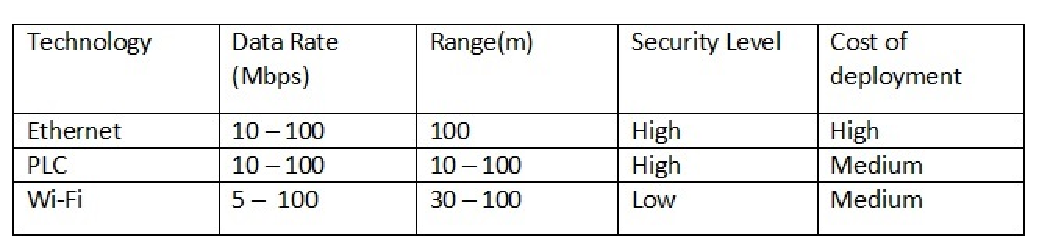
\includegraphics [height=6cm] {HANTechnologies}
\caption{Main technologies used in the HAN Domain}
\label{fig:han}
\end{figure}


\subsection{802.11s}\label{tech::80211s}
TBD
(I removed the RF section. Instead of presenting Wi-Fi directly, it's better to focus on the 802.11s that allows for the multi-hop operation for 802.11 (similar to what you were describing in your RF section)
%Compared to cellular technologies, and advantage of using RF technologies is that these typically use unlicensed bands that do not incur any carrier costs to the Utility. The Utility must only own the terminal units (which in most cases are relatively chep) and could be integrated with the local processors at the Operator side. By using multi-hopping, the range of communication could be extended. Wi-Fi becomes one of the main RF technologies to be used in the NAN domain. When existing feeder infrastructured is re-used to mount multi-hopping points on electric poles, Wi-Fi could be used for long-range communication by multi-hopping from one end to another. By improving receivers and directional antennas, the range issues derived from the very nature of Wi-Fi can be mitigated to some extent.

\subsection{Power Line Communication (PLC)}\label{tech::plc}

PLC is a technology that uses the existing electric grid to transmit data at a maximum rate of 11kbps. PLC becomes a well suited alternative as it is a no-cost medium for the Utility and is spread along the distribution system. Thus, PLC is a natural solution for the communication between the Utility and the Smart Meters. By reusing the electric grid as communication media, the implementation investment is low. In a typical PLC network, the smart meters are connected to the data center through power lines. The main technical specifications of this technology are stated below.

Two main types of communication architectures based on PLC have been defined: NarrowBand PLC (NBPLC) and Broadband PLC (BPLC). The first type allows data transmission at lower rates than those provided by BPLC (from few dozens of kbps to 100 Mbps, respectively) \cite{Sabbah2014}. NBPLC systems generally use the CENELEC (Comité Européen de Normalisation Electrotechnique) bands (3-148.5 kHz). NBPLC generally operates in transmission frequencies of up to 500 kHz, as opposed to BPLC, which targets much higher bandwidth at shorter distances and operates over a much higher frequency band. Frequencies of 148.5 kHz and less have been recognized by CENELEC standards for use in NBPLC systems on a public utility's power wires. Regarding the BPLC, the operation bands go from 1.8 MHz up to 250 MHz. Some examples of NBPLC technologies are described in IEEE 1901 and ITU-T G-hn (G.9960/G.9961) recommendations. NBPLC generally refers to PLC systems supporting data rates over 1 Mbps.

The main advantage of PLC is associated to the low implementation costs. Additionally, the coverage provided by PLC is exactly the one intended by the Utility. As it uses the power feeder, PLC behaves as an enabler for sensing, control, and automation in large systems comprising tens or even hundreds of components spread over relatively wide areas, which contributes to provide scalability. Furthermore, as the power lines are owned by the Utility, there is more independence in relation to sending information through third-party networks or operators. Nonetheless, the very nature of  PLC's physical transmission media generates some challenges. It is highly susceptible to signal degradation due to the harsh power lines. The technology is also limited by its low bandwidth, which is why it may not be suitable for more robust applications where large amounts of data need to be transferred. Besides the fact that feeder cables are not designed for data transmission, they are also prone to be interfered by the inverter’s outcome. %Therefore, PLC modems developed for domestic applications may not be suitable. 

A summary of the technologies used in the NAN domain is depicted in (Fig. \ref{fig:nan}).

\begin{figure}[h!]
\centering
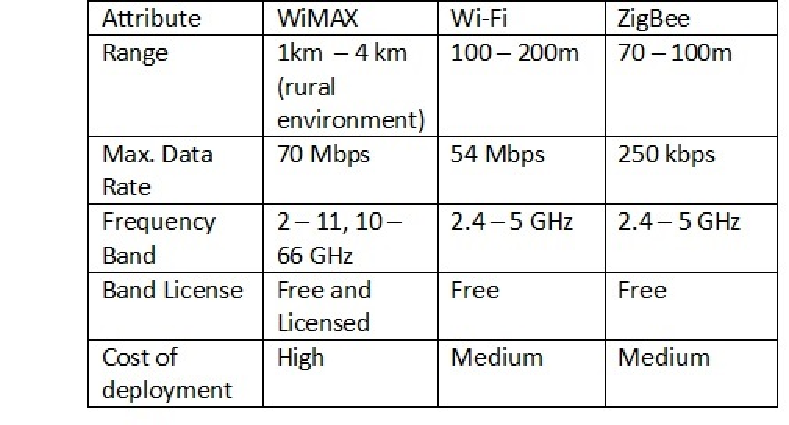
\includegraphics [height=6cm] {NANTechnologies}
\caption{Main technologies used in the NAN Domain}
\label{fig:nan}
\end{figure}


\subsection{Digital Subscriber Lines (DSL)}\label{dsl}
DSL is a high speed digital data transmission technology, which employs the wires of the voice telephone network for data transmission. As with PLC, this technology may be a suitable candidate for the implementation of network segments within the AMI, as it reuses the existing infrastructure, thus reducing installation cost of an implementation from scratch. As for the technical specifications, the network performance and perceived throughput will depend on how far away the subscriber is from the serving telephone  \cite{Gungor2011}. Main technical details, advantages and drawbacks of this technology are listed below:

Technical specifications: Commonly, the frequencies on which this technology works are greater than 1MHz through an ADSL enabled telephone line. 

Advantages:With a high data transmission rate, and given the low installation costs for the network deployment, DSL is a good option for the AMI implementation.

Drawbacks: Distance dependency and lack of standardizations are the primary constraints of this technology.

\subsection{WAN domain}

\subsubsection{Cellular Networks}\label{tech::cellular}
Cellular Networks has been a popular technology for the communication between the smart meters and the Utility (NAN section), as they use the existing infrastructure, thus avoiding incurring in additional installation and deployment costs. However, it is also suitable for communication collectors to the central data center at the Utility's premises. Some of the cellular technologies employed for the long-haul communication are: 2G, 2.5G, 3G, and LTE. The latter has a high-capacity of bandwidth and, consequently, can also support several QoS requirements.

Advantages: When outsourcing the communications network to a mobile operator, utilities can significantly reduce operative costs, as they don’t have to bear the cost of deploying and maintaining the infrastructure. Data rates for cellular technologies-based AMI projects are now much more competitive. On the other hand, coverage provided by cellular networks is another outstanding advantage, which helps to improve network capabilities. Thus, because of the fact that the cellular network infrastructure already exists, the Utility does not have to incur in additional costs for building infrastructure. Due to the significant amount of information that is transported between the Utility and the Client, a large bandwidth capacity is sometimes required (such is the case of 3G, 4G and WIMAX), which is provided by these cellular networks. In general terms, the low maintenance costs and fast installation are the main advantages of this technology. 

Drawbacks: The main drawbacks of cellular networks are associated to information security. As the physical medium used for transmission is susceptible to interceptions, sensitive information (such as contractual data or bills) must be protected, to guarantee that it reaches its intended recipient with no understanding by other individuals or devices attempting to intercept it. On the other hand, particularly given that the communication channel in the SG is shared with users of the mobile telephony, the network performance may be impaired. Finally, in adverse situations such as wind storms, the service could not be guaranteed, neither the communication in the SG. Moreover, transmission through cellular networks still has a high cost, especially when SMS is used as communication media between smart meters and data collectors.While WiMax provides a solution with a large communication range and high data rates, it tends to be costlier due to the greater licensing and subscription fees. 


\subsubsection{WiMAX}\label{tech::wimax}
TBD: PLEASE INCLUDE WIMAX AS A SEPARATE TECHNOLOGY FOR WAN DOMAIN


\section{Routing} \label{routing}

As a first development phase of smart grid involves the implementation of an Advanced Metering Infrastructure (AMI), which is expected to provide a two-way communication path between utilities and consumers, a deployment of a network connecting a dense number of nodes (meters) with data collectors is needed. But most importantly, such mesh based AMI network should provide efficient and suitable routing functionalities, which guarantee a reliable and effective delivery of packets. Regarding the traffic involved in the two-way communication channel, two types of traffic can be identified: 1) inward unicast traffic, consisting of data containing the meter-reading, going from homes to Utilities’ data collectors, and 2) outward unicast traffic, consisting of data containing data going from collectors to substation or the Utility itself. 

The importance behind the implementation of efficient routing strategies and protocols lies in the need of an effective data packet delivery mechanism. It is required that data transmitted between nodes in the WMN reach the final destination (data collector), so that such information can be successfully received by the Utility, through the bidirectional communication channel outlined under the AMI concept. In \cite{Sabbah2014} routing protocols have been classified, according to the AMI component in which they are used (HAN, NAN or N2N). As a consequence, several routing protocols and strategies are specified.


\subsection{RPL}\label{rpl}

In this part of the AMI, the routing protocol must guarantee low energy consumption; assure privacy and information security, as well as supporting self-organization and self-configuration features. For this purpose, IETF has proposed RPL (Routing Protocols for Low Power and Lossy Networks)  \cite{Winter2012}. This protocol is of the distance-vector type, and is based on IPv6. It was designed considering the requirements specified in RFC 5826 \cite{Brandt2010}, RFC 5673 \cite{Pister2009}, RFC 5548 \cite{Dohler2009} and RFC 5867 \cite{Martocci2010}. 

In \cite{Wang2010} , a detailed RPL implementation for AMI networks is presented. The authors considered a static multi-hop wireless AMI network that consists of n meter node and one gateway node. In the proposed protocol, a DAG structure is maintained at the gateway node. Once the information that must be stored and maintained by each node is defined, the data traffic forwarding rules are introduced. Then the authors provided a detailed characterization for the DAG construction and maintenance, as well as an ETX measurement scheme based on MAC layer mechanism. Finally a reverse path recording mechanism is proposed, in order to enable routing support for outward unicast traffic, which flows from the gateway to each meter. 

D. Wang et al \cite{Wang2010} also presented a practical implementation of RPL that aims at providing reliable and low-latency routing support for large-scale AMI networks, through the integration with CSMA-based MAC layer protocols. The authors adopted the Expected Transmission Time (ETX) as the link metric, and proposed a novel ETX-based rank computation method to provide high end-to-end reliability in AMI networks. 

One of the main advantages of this protocol is that it does not define a unique routing metric, but gathers a set of metrics. This is a must in the AMI network, given its heterogeneous and diverse nature. Multiple devices involved in the AMI, as well as the different types of applications uploaded to the network, entails a need to define several types of metrics to ensure the protocol efficiency in all cases. For this purpose, an objective function (OF) is defined, in which a set of metrics are combined. 
The main idea behind RPL is to maintain information about the network status using one or more directed acyclic graphs (DAGs). A DAG is a directed graph in which all edges are oriented in such way that no cycles exist. For each DAG created in RPL there’s a root. The DAG’s root is typically the Gateway in the AMI network. All edges in the DAG are contained in the routes oriented to the root node. Each node in the DAG is associated to a Rank or value. For the construction of the DAG, the Gateway will create control messages called DIOS (DAG Information Object). The main functions executed by the DIO messages are listed below  \cite{Iyer2011a}:


\begin{itemize}
	\item To identify the DAG from which any root is originated
	\item To spread the Rank information of the starting node
	\item To define the objective function (OF) that specifies the metric or the combination of metrics used to compute the Rank in each node.
\end{itemize}

Once multiple DIO messages have been received, a node will compute its own Rank and will determine its position in the DAG. One way to compute the Rank is utilizing ETX (Expected Transmission Count) as a metric. ETX will measure the quality of a route between two nodes, by estimating the average number of required transmissions to send data packets to a neighbor. As nodes in a wireless sensor network (like AMI) are susceptible to multiples faults, RPL builds a Destination Oriented DAG (DODAG) with several routes from each node. This contributes to enhance the performance and robustness of the network, as well as to guarantee quality of service and to handle traffic in real time  \cite{Pavkovic2011}.

\subsection{Geographic routing}\label{geographic}

In this routing principle paths can be discovered through the node coordinates. For this purpose, GPS receivers are required, as well as the use of hard coding. Among the drawbacks of this protocol, we can mention that the GPS devices have a high price, as well as the immediate consequence derived from the use of hard coding, in which the coordinates can’t be changed. This may result in a problem, as consumer’s locations may change. In general terms the determination of geographical location is a challenging task  \cite{Sabbah2014}. 

Gopalakrishnan  \cite{Iyer2011a} presented a performance analysis of Geographical routing in AMI networks, through a simulation set up.  The author considered this protocol because of the fact that it has been widely used in smart utility networks and AMI deployments, currently running in over 2 million metering end-points. For analysis purposes, a 100 node derived from a rurally deployed real AMI network was set up. Several data such as the computed ratio of total transmitted packets to those received by each node, the packet success probability and latency were collected. 

Geographic routing considers packet forwarding by means of position information instead of network addresses and routing tables. The destination location is utilized to route the packet. Through the neighbor’s location, each node can select the next hop that is closer to the destination (specified by its location). One of the main advantages of this routing protocol is that routing tables maintenance and route discovery are unnecessary activities, as the packet forwarding function is only based on geographic information. Three assumptions are required for geographic routing to be performed: i) A node can determine its own position; ii) A node is aware of its neighbor’s positions; and iii) The position of the destination is known \cite{Rührup2009}. 

Regarding the determination of every node’s position, GPS devices are the main tools utilized for making position information available. On the other hand, to enable the node’s awareness of its neighbor’s positions, a broadcasting of the position information to other nodes in the network is required. Finally, in order to determine the position of the destination, a location service mapping network addresses to geographic locations is needed (excepting in cases in which the destination inherently knows the location, like in some sensor network applications, where a node can collect some measurement information). Thus, if a positioning system already exists geographic routing provides a scalable solution for routing in wireless networks.



\subsection{AODV}\label{aodv}

Ad Hoc On-Demand Vector routing protocol builds on the Destination-Sequenced Distance- Vector [DSDV] algorithm and is based on the RFC 3561 \cite{Perkins2003} . AODV creates routes on demand basis by minimizing the number of required broadcasts unlike the DSDV algorithm which maintains a list of routes. This algorithm is an improvement to DSDV algorithm. AODV  is also called as a pure on-demand routing acquisition system because only the nodes  which are on the selected path maintain the routing information are involved in routing  table exchange.  When a source node wants to communicate with some destination node but does not have a valid route to that destination, the source node then initiates a path discovery process to discover the other node. To achieve this, source node broadcasts Route Request [RREQ] packet to its neighbors. This request is in turn sent to its neighbors and so on until either the destination route or an intermediate node route to the destination is traced. This protocol uses hop count as routing metric.

In \cite{Toimoor2013} a test-bed implementation of AODV in an AMI small scale scenario is presented. In the simulation the nodes were placed at distances such that the transmitted signal was only received by the neighboring nodes. As the number of hops increased, the throughput decreased, which is quite obvious due to the routing overheads increment. Regarding the scalability of AODV, it was tested in a large scale string scenario, showing an inverse relationship between the throughput and the number of nodes. A modification of the protocol, where some nodes are provided more intelligente than the others, contributes to lower latency than regular AODV, making it a useful protocol communication for certain current and future AMI applications.


\subsection{DSR}\label{dsr}

Dynamic source routing protocol is an on-demand routing protocol and is based on the concept of source routing. It is based on the RFC 4728 \cite{Johnson2007} . In this protocol, a node maintains a route cache which contains source routes that is known by all other nodes. The route cache is continually updated as new routes to the source are learnt by the nodes. This protocol maintains two major phases: Route discovery and Route maintenance. Whenever a node has to send a packet to some destination, it initially checks the route cache to find out whether the route to the destination is already known. If the route to the destination is already present in the route cache, it uses the same route to transmit the packet. On the other hand, if the route to destination is not present in the route cache, then the node initiates route discovery by broadcasting a route request packet. This route request packet contains destination address, source node’s address and a unique identification number. Each and every node checks if it has the destination route to the address sent in the route request packet. If the node does not find the destination route in its route cache, it adds its own address to the route record packet and forwards the packet to the nodes among its outgoing links. A route reply is generated only when the route request packet reaches the destination or an intermediate node containing the route to the destination in its route cache. 
	
If the route reply is generated by the destination, then the destination places the route record contained in the route request into the route reply. If the route request is responded by an intermediate node, then it will append its cache route to the route record to generate the route reply. The responding node must have a route to the initiator in order to send the route reply. If the responding node has the route to the initiator in its route cache, then it should use that route. Otherwise, if symmetric link is supported, then the node must send the route reply by using the reverse route in the route record. 

\subsection{DADR}\label{dadr}

Distributed Autonomous Depth-First Routing (DADR) \cite{Iwao2009} is a proactive distance vector protocol that uses a control mechanism to provide at most k (if available) paths for each destination. It also utilizes Depth First Search algorithm for path recovery in cases of link failure. As the data forwarding occurs, all the information learned is used to update the routing table. This happens during periodic Hello Messages exchanges among neighboring nodes, or when the nodes receive a route poisoning message. In order to control and detect loops, a unique FID (Frame ID) is added to a packet. Each time a node forwards a packet its FID is stored in the FID table, as well as the packet’s sender and packet’s next hop. Thus, if given a received packet, the node finds its FID in the FID table, it means that a loop is about to occur. When the loop is detected, a poisoning message is generated, so the other nodes in the topology are informed about the situation, making the route to be removed from their routing tables. 

In \cite{Iwao2010} a simulation of scenarios of about 2107 smart meters was run, and an analysis of the routing protocol was tested in a 1500 node network topology. As for the reliability, the protocol shows the capability of learning new routes in both indoor and outdoor environments. On the other hand, the protocol doesn’t need too much control overhead when updating routes, which is an advantage in a large-scale network. Finally, packet latency in a flat mesh network is affected by the several hops the data packet needs to travel forward to in order to reach the destination.

\subsection{HYDRO}\label{hydro}


Hybrid Routing Protocol \cite{Dawson2010} is a link state routing protocol for Low Power and Lossy Networks (LLNs). It uses DAGs to provide multiple reliable paths to a border router. To this end, each node builds its default route table by adding its neighboring nodes towards a  border router. The entries in the route table will be ordered following an ETX metric. According to the top ranked entries of its default table, each node periodically creates a topology report. The nodes piggyback those topology reports on periodic collection traffic, allowing border routers to build and maintain a global view of the topology. The first primitive of HYDRO is the provision of a Default Route Table, which is made of a list of entries (each containing the link-layer address of a node in the direction of a border router). Thus, each node will have information about the link-layer packet success rates, so an evaluation of the quality of that link can be performed. This feature is especially crucial in the reliability requirement, as multiple routes are provided to a given destination. This is why HYDRO is both a centralized and distributed forward mechanism, as low-power nodes maintain a distributed DAG that provides them with a set of default routes for communicating with border routers, which will maintain a global view of the network topology (through the reports sent by each of the nodes). 

In \cite{Dawson2010} a performance evaluation of HYDRO on different metrics was executed through the implementation of a set of testbeds and a real network deployment. In this last one, a 57 node network was set up with HYDRO as the running routing protocol, during six months. The workload consisted of each node transmitting every 1 minute to an external server. The statistics collected show that the PDR is an average 98.9\%. As for the scalability, every node’s state is bound by the number of destinations it communicates with. 

\subsection{Hybrid Wireless Mesh Routing Protocol (HWMP)}\label{hwmp}

The Hybrid Wireless Mesh Protocol (HWMP) is the multihop default routing protocol for IEEE 802.11s WLAN mesh networking. With the purpose of allowing interoperability between devices from different vendors, HWMP serves a common path selection protocol for every IEEE 802.11s compliant device. The term hybrid is due to the use of both reactive and proactive approaches in the routing scheme. HWMP results from an adaptation of AODV called Radio-Metric AODV (RM-AODV), which, unlike AODV, works on layer 2 and uses a radio-aware as routing metric. 

In \cite{Bahr2006} the route discovery process is explained, stating that when a node needs a path to a given destination broadcasts a route request message requesting a route to that destination. This route request message is processed and forwarded by all mesh points to the originator of the route discovery. The destination node or intermediate nodes with a path to the destination answer with a unicast reply message indicating the route requested. Finally the forward path to the destination is set up. 


\section{Metrics used for routing strategies comparison}\label{metrics}

The communication infrastructure in smart grid undertakes important information exchange responsibilities, which are the foundations for the function diversified and location distributed electric power devices to work synergetically. Unsatisfactory communication performance not only limits the AMI from achieving its full energy efficiency and service quality, but also poses potential damages to the grid system. To protect the AMI and ensure optimal operation, the communication infrastructure must meet a number of requirements.

\subsection{Routing strategy}
Depending on the layer in which the routing decision takes place, the data forwarding mechanisms can be classified as mesh-under or route-over. Following sections describe both schemes in more detail.

\subsubsection{Route-over}
In route-over scheme all routing decisions are taken in the network layer where each node acts as an IP router. In route-over, each link layer hop is an IP hop. The IP routing supports the forwarding of packets between these links. In the forwarding process IP routing tables and IPv6 hop-by- hop options are used. For routing and forwarding processes the network layer takes decision using the additional encapsulated IP header. The adaptation layer of 6LoWPAN establishes a direct mapping between the frame and the IP headers. When an IP packet is fragmented by the adaptation layer, fragments are sent to the next hop based on the routing table information. The adaptation layer of the next hop checks received fragments. If all fragments are received successfully, the adaptation layer creates an IP packet from fragments and sends it to the network layer. If the packet is destined for itself, the network layer sends the IP packet to the transport layer, otherwise forwards the packet to the next hop based on the routing table information. If there are one or more fragments missing, then all fragments are retransmitted to one hop distance. After receiving all fragments successfully the adaptation layer creates an IP packet from these fragments and passes it to the network layer. The network layer then forwards or processes the IP packet based on the destination of the packet.

\subsubsection{Mesh-under}
In this scheme, the network layer does not perform any IP routing. The forwarding decision is made at the adaptation layer which forwards the packet to the destination over multiple radio hops. In Mesh-Under scheme, routing and forwarding are performed at link layer based on 802.15.4 frame. To send a packet to a particular destination, 64 bit address or the 16 bit short address is used and sent it to a neighbor node to move the packet closer to the destination. Because multiple hops based on link layers are used to complete a single IP hop, it is called the mesh-under approach. An IP packet is fragmented by the adaptation layer to a number of fragments. On the other hand, these fragments are delivered to the next hop by mesh routing to reach the destination. Different fragments of an IP packet can go through different paths and they are all gathered at the destination. If all fragments are reached successfully, then the reassembling of the IP packet takes place at the adaptation laye. In case of loss of any fragment, the entire IP packet (this is, all fragments for this IP packet) must be retransmitted to the destination for recovery.

\subsection{Availability}

The main objective of this metric is to ensure that network services are available and will survive possible attacks or failures that could occur. In the HAN scenario, for example, resource depletion is typically not a concern when it comes to a resource such as energy, where both the smart meter and appliances are assumed to have access to the grid power. But computation capabilities and memory constraints could be exploited by keeping these resources fully loaded, affecting the ability of the network to function as desired. Equipment failures may also be more common, especially with the low cost of HAN radio (like the ones provided by ZigBee).

\subsection{Latency}
The concept of latency refers to the maximum time in which a particular message should reach its destination through a communication network. It?s important to state that the messages between various entities within the AMI may have different network latency requirements. Thus, while the protection information and commands exchanged between intelligent electronic devices (IEDs) in the distribution network will require a lower network latency, the information messages exchanged between electrical sensors and control centers may accept higher values of latency.  Moreover, the messages exchanged can be event driven (e.g., protection and control related) or periodic (e.g., monitoring related) \cite{Winter2012}. The network architecture and communication medium must support the diverse requirements. The network architecture will determine if the message sent from one communicating entity to the other will reach its destination in one or more hops. This will directly affect the latency. Similarly, the data rates supported by the communication medium also dictate how fast an entity can communicate an event observed or reply to a message received.  The communication technology employed should be able to provide low-latency communications from the data generation or collection point to the eventual destination. Control commands from grid operators should similarly reach smart meters and consumers with minimal delay. For the AMI application, a higher latency may be tolerable for the data collected from smart meters to the control center, but there are control commands in the other direction (from the control center to smart meters) for controlling loads and remote connect/disconnect that may needto communicate immediately.

\subsection{Data delivery}
This refers to the criticality of arrival of packets throughout the network, and it will depend on the needs of the application. This need may be decided at the time of connection establishment between two applications. Different levels of data delivery criticality can be considered, as following: i) high, it is used where the confirmation of end-to-end data delivery is a must and a retry will be mandatory in case of absence of confirmation; ii) medium which is used where end-to-end confirmation is not required but the receiver is able to detect data loss; iii) non-critical, which will be used when data loss is acceptable to the receiver. In this case reliability can be improved by repetitive messages. In this last case, the non-critical level can be used for periodic data for monitoring purposes. 

\subsection{Reliability}
The grid stability will depend, to a great extent, on the reliability of the distribution network. Hence, it becomes extremely important for the communication backbone to be reliable, in order to enable successful and timely message exchanges. Different events may affect the communication backbone reliability. Some of these failures include time-out failures, network failures, and resource failures. A time-out failure occurs if the time spent in detecting, assembling, delivering and taking action in response to a control message exceeds the timing requirements \cite{Wang2011a}. On the other hand, a network failure occurs when there is a failure in one of the layers of the protocol suite used for communication (this is, the failure may be originated in a logical level, and prevent a packet to reach its destination in spite of the existence of a physical link). Other factors can affect the communication, such as noise and interference. Finally, a resource failure implies failure of the end node which initiates communications or receives messages. Hence, there is a need to assess the reliability of the system in its design phase and find ways to improve it.

\subsection{Confidentiality}
The goal of this metric is to ensure that any sensitive data is not disclosed to parties other than those involved in the communication process. The target is that apart from the customer and utility, no other party obtains access to the appliance usage behavior of the customer. Further the customer would prefer the utility to have only an aggregate view of power consumed.

\subsection{Interoperability}
Interoperability of a smart grid is the ability of diverse systems to work together, use the compatible parts, exchange information or e quipment from each other, and work cooperatively to perform tasks. It enables integration, effective cooperation, and the two-way communications proposed in the AMI concept, among the many interconnected elements of the smart grid. NIST, which works as the first International Coordinator for smart grid interoperability, developed a framework that includes protocols and standards for information management to achieve interoperability of smart grid devices and system. In \cite{NIST2010} NIST has developed a three phase approach to identify smart grid standards. Phase 1 addresses the engagement of stakeholders in a participatory public process to identify applicable standards and gaps in currently available standards and priorities for new standardization activities, ending with the final publication of the framework report after public comments have been incorporated. Phase 2 will establish a private-public partnership and form a smart grid interoperability panel to drive longer-term progress. Phase 3 will develop and implement a framework for testing and certification of how standards are implemented in smart grid devices, systems, and processes.

\subsection{Security}
Taking into account that the AMI involves a distribution network that will be spread over large areas, and that the information that will transit throughout that network will be sensitive (as it can involve patterns of consumption from the customer, billing, etc.), the security of data becomes a great matter. Moreover, if a wireless communication medium (like WiFi or Zigbee) is used as part of the communication network, security concerns will be increased given the shared and accessible nature of the medium. Hence, to provide security protection for the AMI, it is important to identify different communication use cases (e.g., demand side management, advanced meter reading, among others.) and thus find appropriate security solutions for each case. As an example of that, we can cite the authorization of access to the real time data and control functions, but in order to prevent spoofing in wide area communications, the use of encryption algorithms may be the right strategy to implement. 

On the other hand, according to the Electric Power Research Institute (EPRI), one of the emergent requirements facing the smart grid development is related to cyber security of systems. As indicated in the EPRI report \cite{EPRI2009}, cyber security is a critical issue due to the increasing potential of cyber attacks and incidents against this critical sector as it becomes more and more interconnected. Cyber security must address not only deliberate attacks, such as from disgruntled employees, industrial espionage, and terrorists, but also inadvertent compromises of the information infrastructure due to user errors, equipment failures, and natural disasters. Vulnerabilities might allow an attacker to penetrate a network, gain access to control software, and alter load conditions to destabilize the grid in unpredictable ways.

\subsection{Time synchronization}
Some of the devices on the AMI need to be synchronized in time. The requirements for time synchronization of a device depend on different factors, such as the criticality of the application. For example, processes involving the measurement of phase units (PMUs) have the strictest need of time synchronization as they provide a real-time measurement of electrical quantities (voltage and current) from the Utility. This is why synchronization becomes an important issue as it involves control of different entities within the distribution network. Other examples of mechanisms that help to achieve time synchronization are the Precision time protocol (PTP), which is defined by the standard IEEE 1588 and provides time synchronization with up to nanosecond precision over Ethernet networks, as well as the Global positioning system (GPS).

\subsection{Scalability}
This metric can be considered as the ability of a system to handle growing amounts of work in an efficient manner \cite{Zhou2012}. Most of the times the concern lies on the load scalability, which is the easiness for a system to increase its resources to accommodate the increasing load. For this purpose, it is necessary to define the specific requirements for scalability in this dimension. In our case, the way how we measure the scalability is regarding the ability of the routing table on a router (meter) scales with the number of nodes of the whole AMI network. It is also important to take into account that scalability is related to a more economically deployable system, and thus costs associated to the deployment of the network must be considered. Summarizing, the network of wireless nodes is expected to be quite large considering the scale of towers from the substation to residential units. The communication architecture must work equally well for a small network as for a large network.


\subsection{Easy of deployment}
This refers to the level of feasibility and easiness with which the network can be deployed utilizing a given routing protocol.  

\subsection{Adaptability}
This refers to the ability of the routing protocol to adapt to different network topologies. 

\section{Performance comparison}

In \cite{Iyer2011a} a performance analysis of RPL and Geographic Routing in a Smart Grid context was executed, taking into account some of the metrics described above. In this analysis,  OMNeT++ was used as the simulation tool to implement the routing algorithms in AMI scenarios, based on real topology networks. RPL was implemented to build the DODAG (Destination Oriented Directed Acyclic Graph) using ETX (Expected Transmission count) as the metric for rank computation. On the other hand, Geographical Routing was modeled using a combination of ETX and geographical proximity to compute routes. Links with a packet success probability of more than 60\% were selected as potential neighbor nodes for each node. The distance between each neighbor node and the destination (collector) was computed using the Euclidean distance formula.  

In the study mentioned above, simulations of RPL and Geographical routing algorithms were run for the 500 node real network with the application layer running a test case for gathering the statistics of hop count and end to end delay. The test case used for the performance analysis was constructed based on the scenario that each of the 500 nodes sends multi-point to point traffic directed towards the collector. The application packet rate was set at 1 packet/second. This was done sequentially to measure individual statistics. All other nodes in the network simply participated in the routing and were not allowed to transmit when one of the nodes was transmitting. Each node transmitted 100 packets with the collector as the destination. An average of 160ms and 173ms of delay were obtained for RPL and Geographical routing, respectively. 

Regarding reliability, it was measured by computing the packet delivery ratio, defined as the total number of received packets at the collector over the total number of packets transmitted by each node. On this matter, RPL showed a constant packet delivery ratio between 98\% and 100\% for each packet and an average of 99.98\% while Geographical routing showed similar performance with an average of 99.30\% \cite{Iyer2011a}.  

Other protocols such as DADR and HYDRO are also analyzed, considering their behavior in testbeds and real deployments, with respect to some of the metrics described before. Both protocols share a route-distribution approach. In  \cite{Iwao2010} a study was conducted to determine how DADR would work in a 1500 node network topology. The results showed that this protocol doesn’t need too much overhead when updating routes, which becomes an advantage in large-scale networks. On the other hand, the capability of learning new routes when link failures occur, as well as removing paths because of possible loops, make the protocol outstanding in the Reliability and Adaptability requirements. Finally, an average 97.8\% PDR was obtained. 

HYDRO, as a combination of both centralized and distributed forwarding mechanisms, shows in  \cite{Dawson2010} a high reliability, as multiples routes are provided to a given destination.  By constantly evaluating the qualities of the links, the protocol becomes robust in the Adaptability requirement, as any change in the topology is detected and the protocol reacts to it. A median PDR of 98,9\% was obtained when examining the performance of the protocol in a 57 node real-world deployment. 
	
A summary of the results explained results in this section can be observed in (Fig. \ref{fig:comparison}). A comparison of the seven routing protocols described, considering the metrics explained in the previous section, is performed. 

\begin{figure}[h!]
\centering
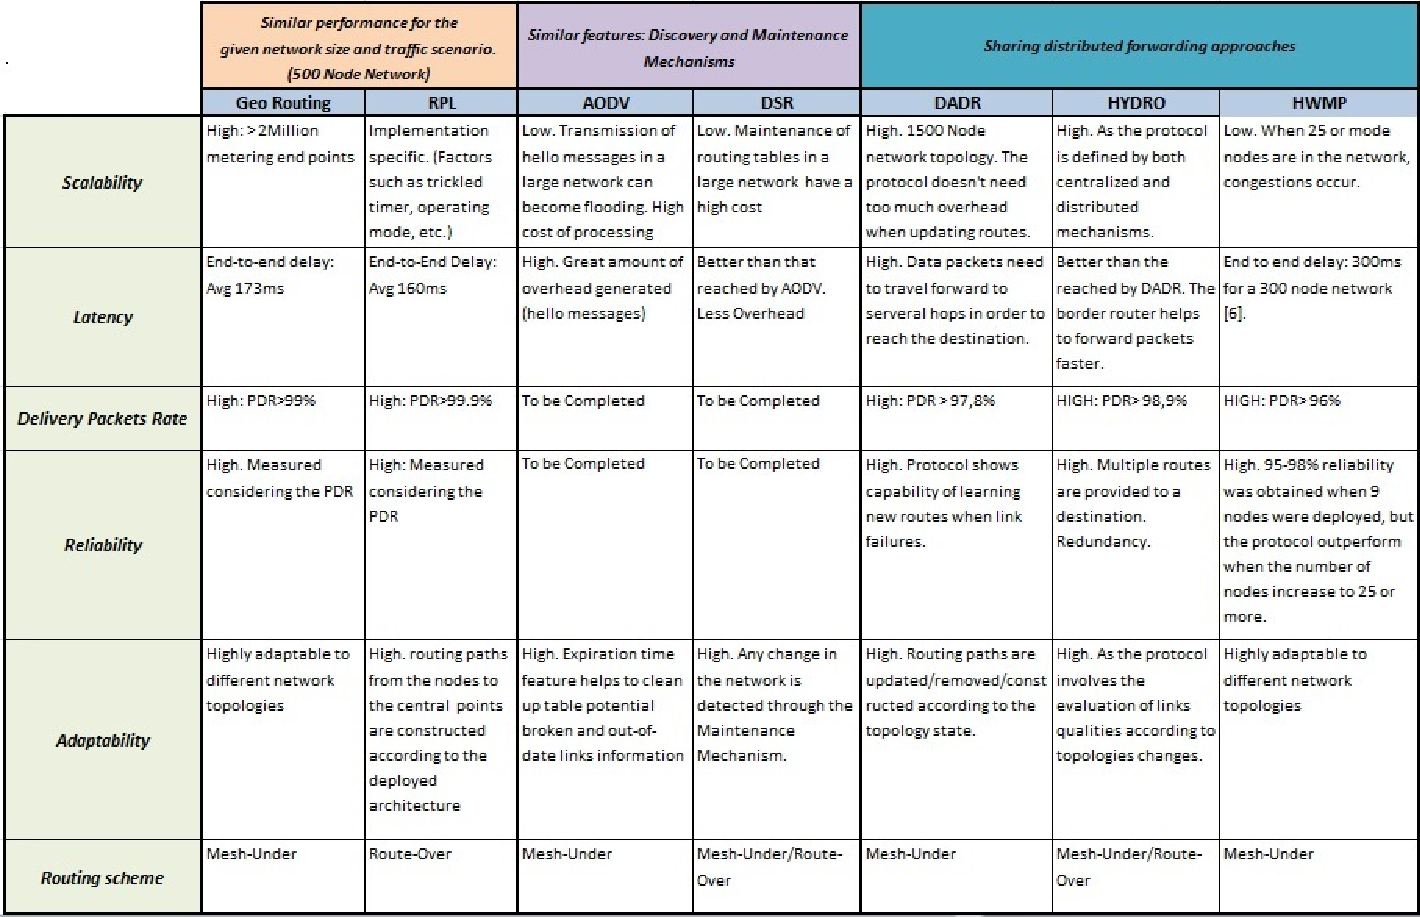
\includegraphics [height=6cm] {comparativeTable}
\caption{Comparison of Routing Protocols in the AMI scope \cite{Wang2010} \cite{Rührup2009} \cite{Perkins2003} \cite{Toimoor2013} \cite{Johnson2007}  \cite{Dawson2010} }
\label{fig:comparison}
\end{figure}

As a primary conclusion, we could say that RPL is most likely to emerge as the imposing protocol as it is on its way to becoming a standard. In order to make this analysis more robust, several other factors such as home, industrial, in-building and outdoor routing conditions and metrics must be considered.

The choice of the routing protocol will then be considered taking into account the technology that is used for deployment purposes. Thus, a protocol might fit better that other, in a certain technology. For instance, in the case of a mesh technology, a protocol that involves end-to-end retransmission when a packet loss occurs wouldn’t be too suitable, as the possibility of fragments loss is bigger in a multihop scheme.



\section{Open Research Issues}\label{issues}
It would be of a great value to test the coexistence of different traffic patterns, which is an important issue, as we mentioned before, given the very nature of the AMI concept. On the other hand the possibility to see tests and evaluations of simulated AMI deployments with real information regarding the energy usage of customers, would also be interesting, as this can have a great impact on the nature of the traffic and its intensity. It will also be an important research issue the determination of the applications that can be supported by each one of the routing strategies defined in this paper, for which different sets of metrics must be defined and evaluated. While meter readings are one of the main features of the AMI, it is also imperative the evaluation of other features and applications that will robust the AMI infrastructure in the near future. It can be concluded that new routing protocols must be designed with various applications in mind, and performance evaluation has to be more comprehensive. Finally, it is important to note that some projects for testing and deployment of SGs in real-world conditions are on the way. For example, Mitsubishi Electric has recently started full-scale tests in Japan on how to manage a large number of renewable energy resources in a power grid. General Motors (GM) and OnStar have also launched projects, in both cases for managing the operation of electric vehicles.


%\appendices
%\section{Proof of the First Zonklar Equation}
%Appendix one text goes here.
%
%% you can choose not to have a title for an appendix
%% if you want by leaving the argument blank
%\section{}
%Appendix two text goes here.
%
%
%% use section* for acknowledgement
%\section*{Acknowledgment}
%
%
%The authors would like to thank...


% Can use something like this to put references on a page
% by themselves when using endfloat and the captionsoff option.
\ifCLASSOPTIONcaptionsoff
  \newpage
\fi



% trigger a \newpage just before the given reference
% number - used to balance the columns on the last page
% adjust value as needed - may need to be readjusted if
% the document is modified later
%\IEEEtriggeratref{8}
% The "triggered" command can be changed if desired:
%\IEEEtriggercmd{\enlargethispage{-5in}}

%references section

% can use a bibliography generated by BibTeX as a .bbl file
% BibTeX documentation can be easily obtained at:
% http://www.ctan.org/tex-archive/biblio/bibtex/contrib/doc/
% The IEEEtran BibTeX style support page is at:
% http://www.michaelshell.org/tex/ieeetran/bibtex/
\bibliography{bibliography_ami_final}
\bibliographystyle{IEEEtran}
% argument is your BibTeX string definitions and bibliography database(s)
%\bibliography{IEEEabrv,../bib/paper}a
%
% <OR> manually copy in the resultant .bbl file
% set second argument of \begin to the number of references
% (used to reserve space for the reference number labels box)
%\bibliographystyle{ieeetr}
%\bibliography{IEEEabrv,}

% biography section
%
% If you have an EPS/PDF photo (graphicx package needed) extra braces are
% needed around the contents of the optional argument to biography to prevent
% the LaTeX parser from getting confused when it sees the complicated
% \includegraphics command within an optional argument. (You could create
% your own custom macro containing the \includegraphics command to make things
% simpler here.)
%\begin{biography}[{\includegraphics[width=1in,height=1.25in,clip,keepaspectratio]{mshell}}]{Michael Shell}
% or if you just want to reserve a space for a photo:

%\begin{IEEEbiography}{Michael Shell}
%Biography text here.
%\end{IEEEbiography}
%
%% if you will not have a photo at all:
%\begin{IEEEbiographynophoto}{John Doe}
%Biography text here.
%\end{IEEEbiographynophoto}

% insert where needed to balance the two columns on the last page with
% biographies
%\newpage

%\begin{IEEEbiographynophoto}{Jane Doe}
%Biography text here.
%\end{IEEEbiographynophoto}

% You can push biographies down or up by placing
% a \vfill before or after them. The appropriate
% use of \vfill depends on what kind of text is
% on the last page and whether or not the columns
% are being equalized.

%\vfill

% Can be used to pull up biographies so that the bottom of the last one
% is flush with the other column.
%\enlargethispage{-5in}



% that's all folks
\end{document}


